\documentclass{beamer}
\usepackage[utf8]{inputenc}
\usepackage{graphicx}
\usepackage{color, colortbl}
%\usetheme{Frankfurt}
\usetheme{Boadilla}
%-------------------TITRE------------------------%
\title{Initiation R}
%---------------Date à remplir ou commenter pour date du jour-------------%
\institute{BiRD}
\date{3 septembre 2013}
\logo{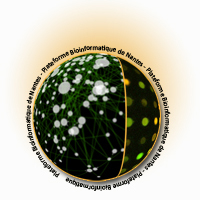
\includegraphics[height=10mm]{image/logo.jpg}}
%--------Rédacteur------------%
\author{E.Hirchaud}

\usepackage{pslatex}
\usepackage{tikz}


\setbeamertemplate{blocks}[rounded]%
[shadow=true]


%Definition de couleur en RGB
%\definecolor{LightRed}{RGB}{255,204,204}
%\definecolor{LightGreen}{RGB}{153,255,153}

\begin{document}

\begin{frame}
	\titlepage
\end{frame}
	

\section*{Sommaire}
\begin{frame}{Sommaire}
	%\tiny \tableofcontents[hideothersubsections]
	\small \tableofcontents
\end{frame}

\section{Notions informatiques}

\subsection{Systéme d'exploitation}
\begin{frame}
	\frametitle{Les systéme d'exploitation : OS (Operating System)}
	\begin{figure}
		
\includegraphics[scale=0.55]{image/OSimage.png}
	\end{figure}
\end{frame}

\subsection{Les applications}
\begin{frame}
	\setbeamercovered{dynamic}
	\frametitle{Les applications : logiciels, programmes, }
	\begin{figure}[h]
		\begin{center}
		  
\includegraphics[scale=0.45]{image/software.png}
		\end{center}
	\end{figure}
\end{frame}


\subsection{Chemins et fichiers}
\begin{frame}
	\frametitle{Arborescence}
	\begin{block}{Appélation}
		\begin{itemize}
			\item Fichiers données numeriques de type variés
			\item Directory = Répertoire = Dossier : contient des fichiers.
		\end{itemize}
	\end{block}
	\begin{columns}
		\begin{column}[c]{5cm}
			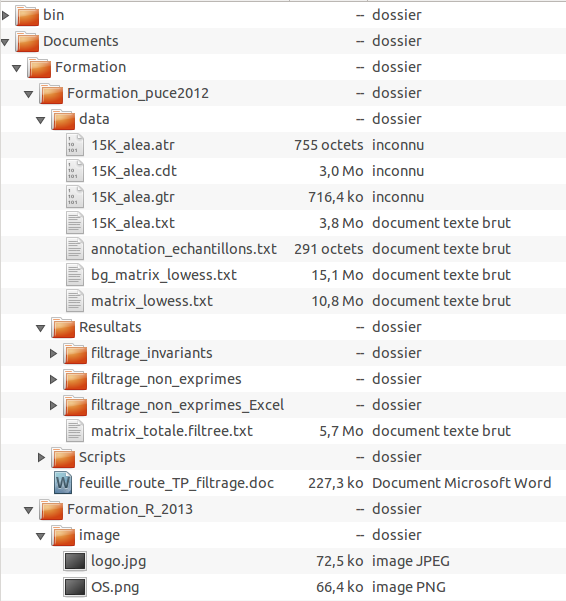
\includegraphics[scale=0.25]{image/ArboUbuntu.png}
		\end{column}
			\begin{column}[c]{5cm}
				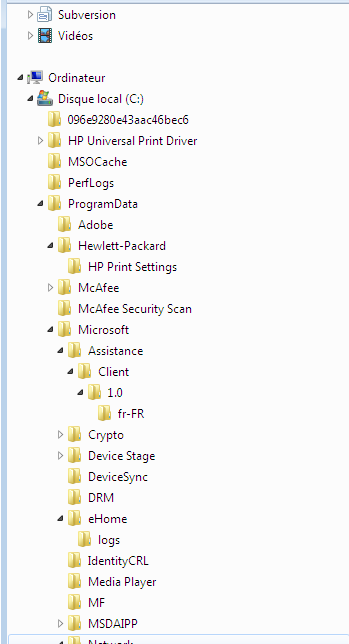
\includegraphics[scale=0.25]{image/ArboWin.png}
			\end{column}
		\end{columns}
\end{frame}

\begin{frame}
		\frametitle{Schématisation}
		\begin{center}
			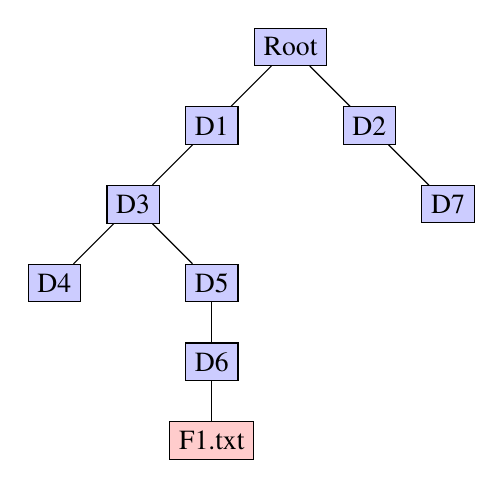
\begin{tikzpicture}[directory/.style={rectangle,draw,fill=blue!20},
				file/.style={rectangle,draw,fill=red!20}]
	\node[directory] (R) at  (0,0) {Root};
	\node[directory] (D1) at (-1,-1) {D1};
	\node[directory] (D2) at (1,-1) {D2};
	\node[directory] (D3) at (-2,-2) {D3};
	\node[directory] (D7) at (2,-2) {D7};
	\node[directory] (D4) at (-3,-3) {D4};
	\node[directory] (D5) at (-1,-3) {D5};
	\node[directory] (D6) at (-1,-4) {D6};
	\node[file] (F1) at (-1,-5) {F1.txt};
	\draw[-] (R) -- (D1);
	\draw[-] (R) -- (D2);
	\draw[-] (D1) -- (D3);
	\draw[-] (D3) -- (D4);
	\draw[-] (D3) -- (D5);
	\draw[-] (D5) -- (D6);
	\draw[-] (D6) -- (F1);
	\draw[-] (D2) -- (D7);
\end{tikzpicture}


		\end{center}
\end{frame}	

\begin{frame}
		\frametitle{La navigation}
		\begin{block}{Deux types de navigation}
			\begin{itemize}
				\item Chemin absolu
				\item Chemin relatif
			\end{itemize}
		\end{block}
		\begin{block}{Symboles utilisés dans la navigation}
			\begin{itemize}
				\item La racine : Windows une lettre, linux et mac, symbole / 
				\item Séparateur de répertoire : Windows : \textbackslash, linux et mac  /
				\item Le Répertoire courrant : . (point)
				\item Le Répertoire parent : .. (deux points)
			\end{itemize}
		\end{block}
\end{frame}

\begin{frame}
		\frametitle{Formalisation : Chemin absolu}
		\begin{columns}
			\begin{column}[l]{5cm}
				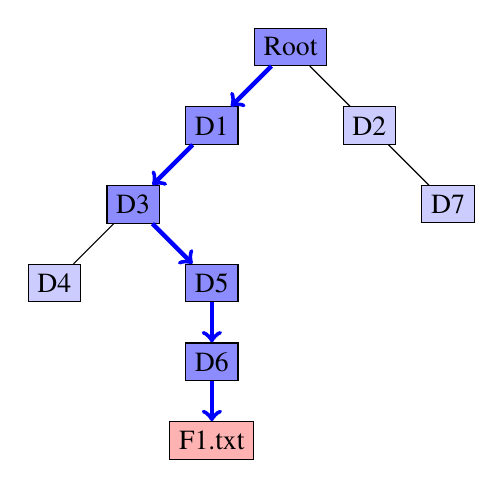
\begin{tikzpicture}[directory/.style={rectangle,draw,fill=blue!20},
					directoryA/.style={rectangle,draw,fill=blue!45},	
	file/.style={rectangle,draw,fill=red!30}]
	\node[directoryA] (R) at  (0,0) {Root};
	\node[directoryA] (D1) at (-1,-1) {D1};
	\node[directory] (D2) at (1,-1) {D2};
	\node[directoryA] (D3) at (-2,-2) {D3};
	\node[directory] (D7) at (2,-2) {D7};
	\node[directory] (D4) at (-3,-3) {D4};
	\node[directoryA] (D5) at (-1,-3) {D5};
	\node[directoryA] (D6) at (-1,-4) {D6};
	\node[file] (F1) at (-1,-5) {F1.txt};
	\draw[->, color=blue, ultra thick] (R) -- (D1);
	\draw[-] (R) -- (D2);
	\draw[->, color=blue ,ultra thick] (D1) -- (D3);
	\draw[-] (D3) -- (D4);
	\draw[->, color=blue,ultra thick] (D3) -- (D5);
	\draw[->, color=blue,ultra thick] (D5) -- (D6);
	\draw[->,color=blue,ultra thick] (D6) -- (F1);
	\draw[-] (D2) -- (D7);
\end{tikzpicture}


			\end{column}
			\begin{column}[r]{5cm}
				\begin{block}{Chemin absolu}
					\begin{itemize}
						\item A partir de la racine (C:)
						\item Root/D1/D3/D5/D6/F1.txt
					\end{itemize}
				\end{block}
			\end{column}
		\end{columns}
\end{frame}

\begin{frame}
		\frametitle{Formalisation : Chemin relatif exemple 1}
		\begin{columns}
			\begin{column}[l]{5cm}
				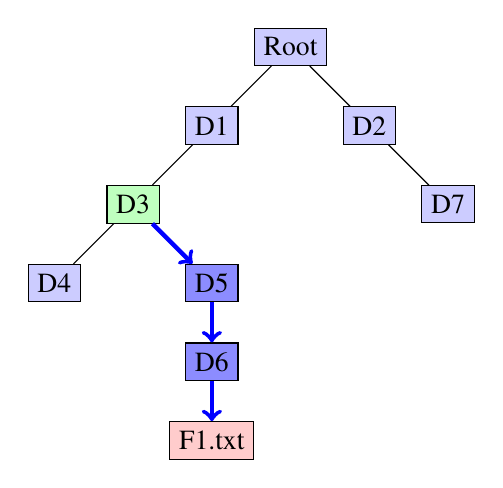
\begin{tikzpicture}[directory/.style={rectangle,draw,fill=blue!20},
				file/.style = {rectangle, draw, fill=red!20},
				directoryC/.style={rectangle, draw, fill=green!25},
				directoryR/.style={rectangle, draw, fill=blue!45}]
	\node[directory] (R) at  (0,0) {Root};
	\node[directory] (D1) at (-1,-1) {D1};
	\node[directory] (D2) at (1,-1) {D2};
	\node[directoryC] (D3) at (-2,-2) {D3};
	\node[directory] (D7) at (2,-2) {D7};
	\node[directory] (D4) at (-3,-3) {D4};
	\node[directoryR] (D5) at (-1,-3) {D5};
	\node[directoryR] (D6) at (-1,-4) {D6};
	\node[file] (F1) at (-1,-5) {F1.txt};
	\draw[-] (R) -- (D1);
	\draw[-] (R) -- (D2);
	\draw[-] (D1) -- (D3);
	\draw[-,] (D3) -- (D4);
	\draw[->, color = blue, ultra thick] (D3) -- (D5);
	\draw[->, color = blue, ultra thick] (D5) -- (D6);
	\draw[->, color = blue, ultra thick] (D6) -- (F1);
	\draw[-] (D2) -- (D7);
\end{tikzpicture}


			\end{column}
			\begin{column}[r]{5cm}
				\begin{block}{Chemin relatif}
					\begin{itemize}
						\item D5/D6/F1.txt
					\end{itemize}
				\end{block}
			\end{column}
		\end{columns}
\end{frame}

\begin{frame}
		\frametitle{Formalisation : Chemin relatif exemple 2}
		\begin{columns}
			\begin{column}[l]{5cm}
				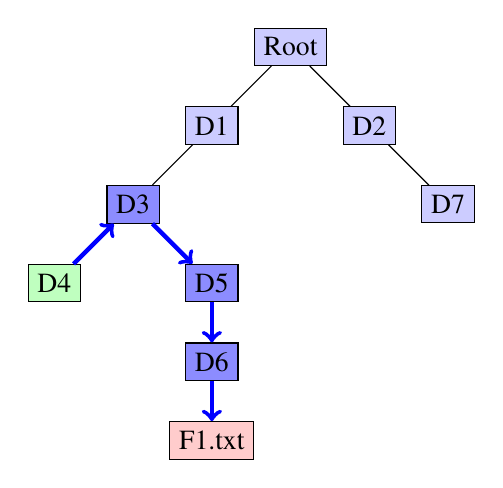
\begin{tikzpicture}[directory/.style={rectangle,draw,fill=blue!20},
				file/.style = {rectangle, draw, fill=red!20},
				directoryC/.style={rectangle, draw, fill=green!25},
				directoryR/.style={rectangle, draw, fill=blue!45}]
	\node[directory] (R) at  (0,0) {Root};
	\node[directory] (D1) at (-1,-1) {D1};
	\node[directory] (D2) at (1,-1) {D2};
	\node[directoryR] (D3) at (-2,-2) {D3};
	\node[directory] (D7) at (2,-2) {D7};
	\node[directoryC] (D4) at (-3,-3) {D4};
	\node[directoryR] (D5) at (-1,-3) {D5};
	\node[directoryR] (D6) at (-1,-4) {D6};
	\node[file] (F1) at (-1,-5) {F1.txt};
	\draw[-] (R) -- (D1);
	\draw[-] (R) -- (D2);
	\draw[-] (D1) -- (D3);
	\draw[<-, color = blue, ultra thick] (D3) -- (D4);
	\draw[->, color = blue, ultra thick] (D3) -- (D5);
	\draw[->, color = blue, ultra thick] (D5) -- (D6);
	\draw[->, color = blue, ultra thick] (D6) -- (F1);
	\draw[-] (D2) -- (D7);
\end{tikzpicture}


			\end{column}
			\begin{column}[r]{5cm}
				\begin{block}{Chemin relatif}
					\begin{itemize}
						\item ../D3/D5/D6/F1.txt
					\end{itemize}
				\end{block}
			\end{column}
		\end{columns}
\end{frame}

\subsection{Types de mémoires}
\begin{frame}
		\frametitle{Les mémoires}
		\begin{columns}
		  \begin{column}[c]{5cm}
		    \begin{figure}[h]
		      \begin{center}
			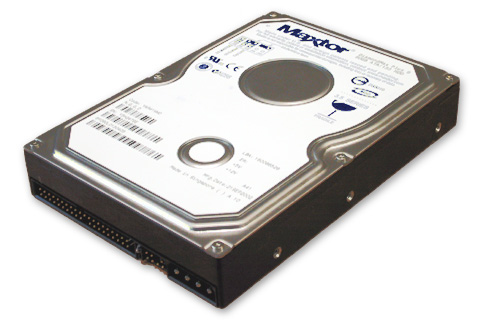
\includegraphics[scale=0.35]{image/hdd.jpg}
		      \end{center}
		    \end{figure}
		  \end{column}
		  \begin{column}[c]{5cm}
		    \begin{figure}[h]
		      \begin{center}
			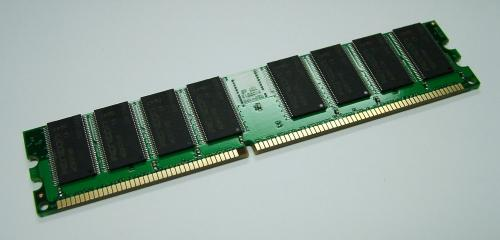
\includegraphics[scale=0.40]{image/memory_chip.jpg}
		      \end{center}
		    \end{figure}
		  \end{column}
		\end{columns}
\end{frame}

 \subsection{Synthèse}
\begin{frame}
	  \setbeamercovered{dynamic}
	  \frametitle{Synthèse}
	  \begin{figure}[h]
	    \begin{center}
	      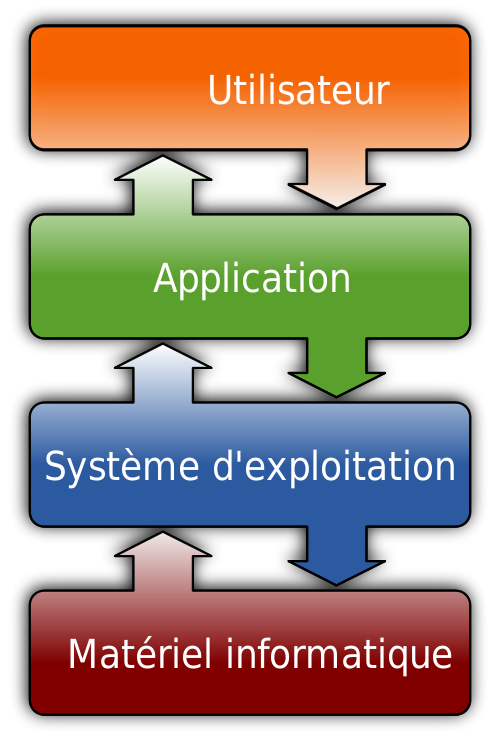
\includegraphics[scale=0.25]{image/OS.png}
	    \end{center}
	  \end{figure}
\end{frame}




\section{R}
\subsection{Apperçu}

\begin{frame}
	\frametitle{R : Apperçu}
	\begin{center}
		\begin{block}{}
			\begin{itemize}
				\item Crée par Ross Ihaka et Robert Gentleman (1996)
				\item C'est un logiciel libre et gratuit
				\item Il est basé sur le langage S qui est propriétaire
				\item Disponible sur les systèmes d'exploitation les plus utilisés
				\item Utilisé dans de nombreux domaines dont la bio analyse.
			\end{itemize}
		\end{block}
	\end{center}
\end{frame}

\subsection{Objectif du TP}
\begin{frame}
	\frametitle{Objectif du TP}
	\setbeamercovered{dynamic}
		
	\begin{itemize}[<+->]
		\item {Assimiler le vocabulaire }
		\item {Se servir de R comme d'une calculatrice}
		\item {Écrire et modifier des lignes de commande}
		\item {Utiliser un script déjà écrit}
		\item {Savoir où trouver de l'aide (documentation)}
		\item {Utiliser un éditeur convivial (RStudio)}%
	\end{itemize}
\end{frame}

\subsection{Comparaison Excel R}
\begin{frame}
	\frametitle{Comparaison Excel R}
	\setbeamercovered{dynamic}
	\begin{center}
		\setlength\doublerulesep{3pt}
		\doublerulesepcolor{blue!15}
	\begin{tabular}[h]{|c||c|}
		\hline
		Excel & R \\
		\hline \hline
		\rowcolor{green!25}
		Cellule & Variable (simple) \\
		\hline
		\rowcolor{green!25}
		Plage de données & data.frame matrix, list, vector \\
		\hline
		\rowcolor{green!15}
		Valeur & Valeur (value) \\
		\hline
		\rowcolor{green!15}
		Format & Type \\
		\hline
		\rowcolor{blue!25}
		Fonction & Fonction \\
		\hline
		\rowcolor{red!25}
		Macro & Script \\
		\hline
	\end{tabular}
	\end{center}
\end{frame}

\begin{frame}
	\frametitle{Généralité sur les variables}
	\setbeamercovered{dynamic}
	\begin{itemize}
		\item Un nom
		\item Valeur(s)
		\item Les valeurs ont un type : 
			\begin{itemize}
				\item numérique : 1,2, 3.14
				\item chaine de caratères : A,B genes
				\item logique : TRUE/FALSE
			\end{itemize}
	\end{itemize}
\end{frame}

\begin{frame}
	\frametitle{Catégories de variables}
	\setbeamercovered{dynamic}
%	\begin{center}
		\begin{itemize}[<+->]
			\item vector $\Rightarrow$ vecteur (type homogène)
			\item matrix $\Rightarrow$ matrice (type homogène)
			\item data.frame $\Rightarrow$ tableau de données (type hétèrogène)
			\item factor $\Rightarrow$ classe de paramètres (type homogène)
			\item list $\Rightarrow$ liste( type hétèrogène)
		\end{itemize}
%	\end{center}
\end{frame}

\begin{frame}
	\frametitle{Les Fonctions}
	\setbeamercovered{dynamic}
	\begin{center}
		\begin{itemize}
			\item Créent, modifient et informent sur les données
			\item Contiennent des arguments et des instructions
		\end{itemize}
	\end{center}
\end{frame}

\begin{frame}
	\frametitle{Règles de nomenclatures}
	\setbeamercovered{dynamic}
	\begin{itemize}
		\item Importance de la casse (majuscule/minuscule)
			\begin{itemize}
				\item : pizza  $\neq$ Pizza
			\end{itemize}
		\item Informatique anglo-saxone
			\begin{itemize}
				\item Ne pas nommer les noms des objets avec des acents
				\item Le point sert de décimal, la virgule non !
			\end{itemize}
		\item Ne JAMAIS mettre d'espace dans un nom
		\item Ne JAMAIS commencer un nom par un chiffre
		\item Eviter d'utiliser des symboles (+ - / \dots)
	\end{itemize}
\end{frame}
\end{document}
